\chapter{System Description}\label{chap:sys_description}
The present chapter covers the system design including specific solutions that have been chosen for the realization of the SmartNotes application. The system concept, introduced in Chapter~\ref{chap:concept}, will become extended by describing certain elements of implementation and problems found during the development process. This should allow the reader to have a deeper view into the SmartNotes application, including the functions that it offers as well as the platform that it runs on.
\section{Google App Engine platform}\label{sec:gae}
Google App Engine seems to be an outstanding development platform. For all the reasons mentioned in~\ref{sec:gae_general}, it has been decided to be used as the main platform for SmartNotes as the one preceding any other hosting services. Besides, GAE appears to be highly competitive in terms of cost calculations, which are described in Section~\ref{subsec:gae_calculations}. After registering the application with a unique name, it can be easily uploaded to Google and after a few seconds it is accessible to its users.

As stressed in Section~\ref{subsec:sync_scenarios}, synchronization scenarios use the client-server architecture. When running on GAE platform which is, as mentioned in~\ref{sec:gae_general}, a distributed vault-tolerant infrastructure where two subsequent request may be served by different machines located in separate data centres. Thus in the addressing scope, the application can still be treated as a centralized server. In case the application requires state awareness, it is the developer's role to make it so. Otherwise, the fact that the application is served from multiple machines is completely transparent from the functional point of view.

SmartNotes uses only some of the components supported by GAE and the ones which make a part of the SmartNotes application with relation with other third-party elements are presented in Figure~\ref{fig:smartnotes_components}. This is especially important as it presents all the application top level components together with marked interfaces between the particular functional blocks. This particular diagram strongly corresponds with the diagram from Figure~\ref{fig:ismartnotes_smartnotes}, which in a more general way presents the cooperation of SmartNotes and iSmartNotes with differentiated roles of the administrator and the user. 

The most complicated structure is the SmartNotes component, which is marked as an individual system. It does not require the iSmartNotes to realize its functionality. For this reason, the SmartNotes component could work with any kind of client application using the interface that the tool provides, or the interface of Mercurial HTTP chains of requests and responses that needed a back-end redesign to accommodate conditions set by GAE. The issues connected with the cooperation of Mercurial and GAE are the topic of Section~\ref{sec:hg_on_gae}. 

Furthermore, SmartNotes uses three additional interfaces which are used to interconnect the Google App Engine component with Mercurial adopted to run on GAE as well as separately, admin and user interfaces provided by SmartNotes. Each of the three components is connected in a different way. Whereas the webapp framework has a low Python overhead as mentioned in Section~\ref{subsec:webapp} and was chosen to serve the connection between the Mercurial and the Google App Engine componet, for performance reasons, it is Django which is the best choice when it comes to building nontrivial web-based functionality for reasons mentioned in Section~\ref{subsec:django}. The remaining two elements used by the GAE subsystem are the Google Account and the Datastore. The role of the first one has been presented in detail while discussing the iSmartNotes activation process in Section~\ref{subsec:ismartnotes_activation}. Some of the Datastore details will be covered in Section~\ref{sec:hg_on_gae}. 
\begin{figure}[ht]
\begin{center}
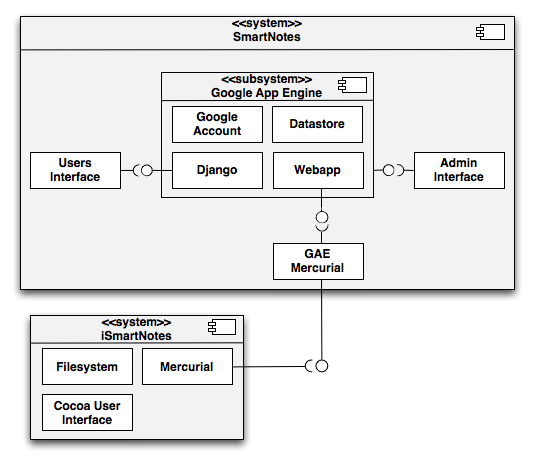
\includegraphics[scale=0.6]{charts/smartnotes_componets.png}
\caption{The components diagram of the SmartNotes application with marked interfaces between the functional blocks.}
\label{fig:smartnotes_components}
\end{center}
\end{figure}

The second independent system is the iSmartNotes component, which remains independent until the user decides to activate it to use the synchronization feature. For this purpose, it requires a Mercurial server to interact with. The iSmartNotes, as presented in Figure~\ref{fig:smartnotes_components}, is build with three components. Firstly, the file system of the client's operating system which is the classical space where VCSs allocate their repositories. Secondly, Mercurial VCS which on the client site does not require any modifications. Finally, the Cocoa user interface whose presentation is provided in Section~\ref{sec:cocoa}.

\subsection{Financial calculations}\label{subsec:gae_calculations}
The role of this section is to introduce some basic calculations that should give the reader a general experience of what kind of resources will be used by the application with the connection to the billing rates set by Google. In the next step this values will be used to predict the order of size for monthly cost of running the application for  one million of SmartNotes users. This should should help to indicate the system elements that generate highest price of resource usage what in the end lets to concentrate on optimization in those specific area. 

Calculations bellow aim to predict theoretical monthly cost of running SmartNotes applications for one million of users with unit price detailed in Table~\ref{tab:gae_cost}. Each of resources will become briefly introduced with short explanation of taken assumptions. The outcome of this considerations is illustrated in Figure~\ref{tab:gae_cost}.
\begin{table}[h]
\centering
\caption{Google App Engine billing rates on September 2009.}
\label{tab:gae_cost}
\begin{tabular}{|l|l|l|} \hline \hline
\textbf{Resource} & \textbf{Unit} & \textbf{Unit cost} \\ \hline \hline
Outgoing Bandwidth & Gigabytes & \$0.12 \\ \hline
Incoming Bandwidth & Gigabytes & \$0.10 \\ \hline
CPU Time & CPU hours & \$0.10 \\ \hline
Stored Data & Gigabytes per Day & \$0.005 \\ \hline
Recipients Emailed & Recipients & \$0.0001\\ \hline \hline
\end{tabular}
\end{table}

Resource usage to price calculations:
\begin{itemize}
\item{\textbf{Outgoing Bandwidth}. This value represents a summarized amount of data send from the server to the users. That normally includes html, css, java script and graphic files as the standard web pages components. In classical case a total size of a web page is round \mbox{70--150KB} what with compression can reduce it by factor of about 40\%. In case of SmartNotes application the content sent between the server and iSmartNotes are the changesets. It was assumed that the size of average downstream changeset won't exceed 2KB. It is smaller from the upstream changeset as not all server responses contain a changeset. A changset is sent only if there is a need for it what happens when there application encounters differences requiring to be synchronized.   

Next made assumption regards the users activity. As stated in the beginning the calculations are done for one million of users. Additionally among this users there is a strong group of active users what translated into numbers would mean that about 80\% of users generate four editing actions. This accordingly to the synchronization scenario from Figure~\ref{fig:seq_commit} might require sending the data from and to the server.  For this reason the the bandwidth calculations for incoming and outgoing traffic use the same number of requests. This all leads to the fallowing numbers:

$Outgoing\ Bandwidth =  80\% \cdot 1,000,000\ users \cdot 4\ requests\ per\ user \cdot$\\ \hspace*{37mm} $2KB\ per\ request \cdot 30\ days \approx \textbf{183GB\ per\ month}$ \\ 
$Outgoing\ Bandwidth\ Cost = 183GB\ per\ month \cdot \$0.12\ per\ GB \approx \textbf{\$22 per\ month}$ }

\item{\textbf{Incoming Bandwidth}. In this case the same number of requests will be used just as in case of outgoing bandwidth. That is 3,200,000 of requests per day and it will be used as basic parameter in all of undermentioned calculations. 

The size of a single request will be double the value taken when calculating the outgoing bandwidth. This is cause each of the operations done by use of iSmartNotes requires sending a changeset. Remaining part of calculations regarding incoming bandwidth follows the numbers which were used for outgoing bandwidth:

$Incoming\ Bandwidth =  3,200,000\ requests\ per\ day \cdot 4KB\ per\ request \cdot 30\ days$\\ \hspace*{33mm} $\approx \textbf{366GB\ per\ month}$ \\ 
$Incoming\ Bandwidth\ Cost = 366GB\ per\ month \cdot \$0.1\ per\ GB \approx \textbf{\$37 per\ month}$ }

\item{\textbf{CPU Time}. This calculation was done by checking the average time that the CPU was idle during serving a single request. As mentioned in Section~\ref{subsec:webapp} has lower Python overhead and for performance reasons it was chosen over the Django framework. This in consequence allowed to reduce the CPU time parameter. Due to the fact that all requests require CPU time the base number of 3,200,000 requests per day is multiplied by two for upstream and downstream requests. Turning that into numbers gives:

$CPU\ Time =  3,200,000\ requests\ per\ day \cdot 2 \cdot 0.02\ seconds\ per\ request \cdot 30\ days$\\ \hspace*{17mm} $\approx \textbf{1067\ hours\ per\ month}$ \\ 
$CPU\ Time\ Cost = 1067\ hours\ per\ month \cdot \$0.1\ per\ hour \approx \textbf{\$107 per\ month}$}

\item{\textbf{Stored Data}. To help imagine the storage space needed for an average notes repository let say that the popular collection of stories called "Winnie-the-Pooh" contains about 4,000 lines and it size in plain text without graphics is about 150KB. When using Version Control Systems it should be remembered as it was mentioned in Section~\ref{subsec:hg} that this systems consume additional disk space. The fudge factor saying how may times the final repository  size will be greater from the its base content size is about 3--4 times. That depends on how many files are stored in that repository and how frequent the changes are. Altogether assuming a size of 1MB for user repository seems to be reasonable and will make the calculations simple.

$Stored\ Data =  1,000,000\ users\cdot 1MB\ per user \cdot 1\ month \approx \textbf{977GB\ per\ month}$ \\ 
$Stored\ Data\ Cost = 977GB\ per\ month \cdot \$0.15\ per\ GB\ per\ month \approx \textbf{\$146 per\ month}$}

\item{\textbf{Mail}. In case of iSmartNotes activation there is no need to send mails to users like in a case of classical account creation what was discussed in Section~\ref{subsec:ismartnotes_activation}.On the other hand mail remains a very effective way to communicate with users. Although they are other possibilities like twitter\footnote{Twitter is an micro-blogging application allowing to share ideas and live-stream informations in the macro scale by the use of Internet.}, placing information on a web page or displaying dialog windows from the application, mailing users with the information remains more solid and professional attempt. For that reason it seems to be worth to take mailing service into account for keeping the users updated just as for sending invitations to potential new users. The additional 20\% of mails send is reserved just for that purpose --- allowing satisfied users to share the information about SmartNotes with their contacts.

$Mail =  1,000,000\ users\cdot (1 + 20\%) = \textbf{1,200,000\ mails\ per\ month}$ \\ 
$Mail\ Cost = 1,200,000\ mails\ per\ month \cdot \$0.0001\ per\ mail = \textbf{\$120 per\ month}$}
\end{itemize} 

This all together encloses in about \$312 without mailing and about \$432 with mailing service. Beside this the application may use the free quota up to limits which are shown in Table~\ref{tab:gae_free}. The free quota resources should allow to reach a rate of 5 million page views per month what could be used to serve the SmartNotes  homepage or as some backup resources for the application. 
\begin{table}[h]
\centering
\caption{Google App Engine free quota limitations on September 2009.}
\label{tab:gae_free}
\begin{tabular}{|l|l|} \hline \hline
\textbf{Resource} & \textbf{Daily Limit} \\ \hline \hline
Outgoing Bandwidth & 1 Gigabyte \\ \hline
Incoming Bandwidth & 1 Gigabyte \\ \hline
CPU Time & 6.5 CPU hours \\ \hline
Stored Data & 1 Gigabyte \\ \hline
Recipients Emailed & 2000 \\ \hline \hline
\end{tabular}
\end{table}

Prior calculated figures could be compared to some popular hosting services like Rackspace, Joyent or Amazon Web Services that offer same resources for prices that are gathered in Table~\ref{tab:services_price_compare} . 
Some services like Joyent or Rackspace are were using some other pricing strategy by using base service price with predefined resources and allowing user to extend it by ordering additional resources. Because of this it is hard to make objectively compare resources prices in separate thus more accurate is to concentrate on the vales presented in Table~\ref{tab:services_price_compare} \emph{Summary} rows.    

Disregarding pricing differences it should be stressed that Google App Engine is not only a hosting service but also exposes for wide use Google infrastructure components that were mentioned in Section~\ref{sec:gae_general} . Furthermore developers which decide to use Google App Engine get access to a bunch of useful API's such as Memcache or URLfetch. Finally the dashboard not only gives a clear view on the application status but also lets to flexibly control the expanses. It allows to set a daily budget that might be changed anytime during the day. When some capital becomes unused it will be available in the next days. On the other hand applications using Google App Engine are protected  from running out of resources by load peaks\footnote{This effect is has a popular name, it is said that application become \emph{slashdoted} what might be the result of placing link to an application on some highly popular social web services like \url{slashdot.org} from which the effect takes name or becoming a target of malicious scripts or load testing programs.}. For all those reasons Google App Engine seems to be not only the most developer friendly and flexible platform but also offering a highly competitive pricing policy.   

\begin{table}[h]
\centering
\caption{SmartNotes resource prices among different hosting providers.}
\caption*{ $^{*}$ This prices couldn't be listed as some services use predefined resource sets and allow to bay extra resources.\\
 $^{**}$ This prices were calculated by using extra bandwidth and CPU time as mailing is not separately billed by those services. That was done by taking following constants: $Average\ Mail\ Size = 100KB$, $CPU\ Time\ per\ 100\ Mails = 0.01s$\\
 $^{***}$ This prices does mot include mail service as it is supplementary for SmartNotes application.}
\label{tab:services_price_compare}
\begin{tabular}{|l|l|l|l|l|l|} \cline{3-6}
		  \multicolumn{2}{c|}{}       &\multicolumn{4}{c|}{\textbf{Resource Price by Service}} \\ \hline \hline
\textbf{Resource} &\textbf{Quantity} &\textbf{Google}        &\textbf{Amazon}         &\textbf{Joyent} &\textbf{Rackspace} \\ 
			     &			   &\textbf{App Engine} &\textbf{Web Services} &           &  \\ \hline \hline
Bandwidth &550 Gigabytes &\textbf{\$59} &\$68 &$^{*}$ &\$69 \\ \hline
CPU Time &1067 Hours &\$107 &\$170 &$^{*}$  &\textbf{\$48}\\ \hline
Stored Data &977 Gigabytes &\$146 & \$216 &\textbf{\$15} &\$146 \\ \hline
Mail &1,200,000 Mails &\$120 &\textbf{\$20}$^{**}$ &$^{*}$ &\$26$^{**}$ \\ \hline \hline
\multicolumn{2}{|c|}{\textbf{Summary}} &\$432 &\$474 &\$1000$^{*}$+\$15 &\$100$^{*}$+\$289=\textbf{\$389}\\ 
\multicolumn{2}{|c|}{} &\textbf{\$312}$^{***}$ &\$454$^{***}$ &(\$1000$^{*}$+\$15)$^{***}$ &\$100+\$263=\$363$^{***}$\\ \hline \hline
\end{tabular}
\end{table}

Presented bellow charts in Figure~\ref{fig:gae_cost} can be used to indicate the resources that usage costs most. From the visualized proportion it is clear that bandwidth is not that an issue as storage, mailing or the CPU time. When mailing service as mentioned before remains supplementary by making some optimization on storage the price could become reduced. One of possible ways is to reduce the history size that is stored with the notes repository. By creating a queue task\footnote{This is one of the Google App Engine features that was introduced in Section~\ref{sec:gae_general} that allows to run tasks in background when the system is not busy.} that would reorganize the SmartNote repositories to store only 20 most recent changsets the repository size might get reduced up to 50\%.      

\begin{figure}[ht]
  \begin{center}
    \subfigure[\textbf{Without mailing service}.]{\label{fig:gae_cost_without_mail}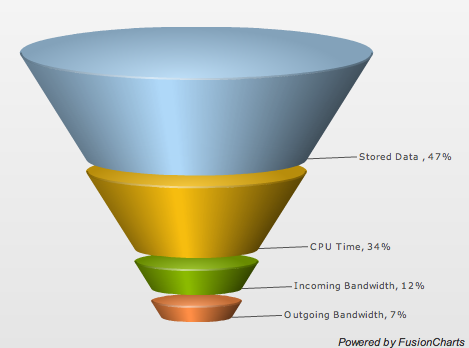
\includegraphics[scale=0.45]{img/price_div.png}}
    \subfigure[\textbf{With mailing service}.]{\label{fig:gae_cost_with_mail}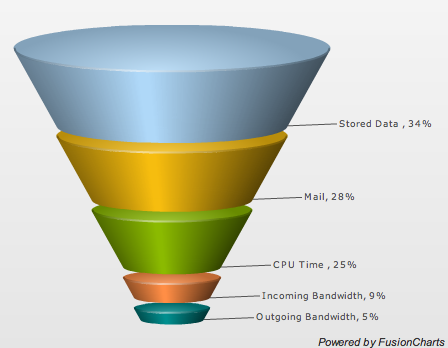
\includegraphics[scale=0.45]{img/price_div_mail.png}}
  \end{center}
  \caption{Simulated monthly cost division of resources expected to be used by one million of SmartNotes users on Google App Engine.}
  \label{fig:gae_cost}
\end{figure}


\section{Mercurial on Google App Engine}\label{sec:hg_on_gae}
\section{Cocoa user interface}\label{sec:cocoa}
